% slides.tex
\documentclass[20pt]{beamer}
\usepackage{listings}
\usepackage[utf8]{inputenc}
\usepackage{color}
\usepackage{graphicx}

\usetheme{default}
\usecolortheme{dove}
\useoutertheme{default}

% Slightly smaller title
\setbeamerfont{frametitle}{size=\large}
\setbeamerfont{verb}{size=\small}

% lst settings
\lstset{
    language=Haskell,
    basicstyle=\small,
    gobble=4
}

\newcommand{\vspaced}{
    \vspace{5mm}
}

\begin{document}

\title{\texttt{tsuruCapital :: \\
    Lambda -> Dollar}}
\subtitle{FLP 2012}
\author{Jasper Van der Jeugt}
\date{December 12, 2012}

\begin{frame}[plain]
    \titlepage
\end{frame}

% Introduction
% ------------

\begin{frame}{Hello!}
    My name is Jasper \\
    Student at UGent \\
    I write Haskell \\
    Tsuru Capital \\
    \texttt{@jaspervdj} \\
    \texttt{jaspervdj.be}
    \begin{picture}(0.0, 0.0)
    \put(30.0, -35.0){
        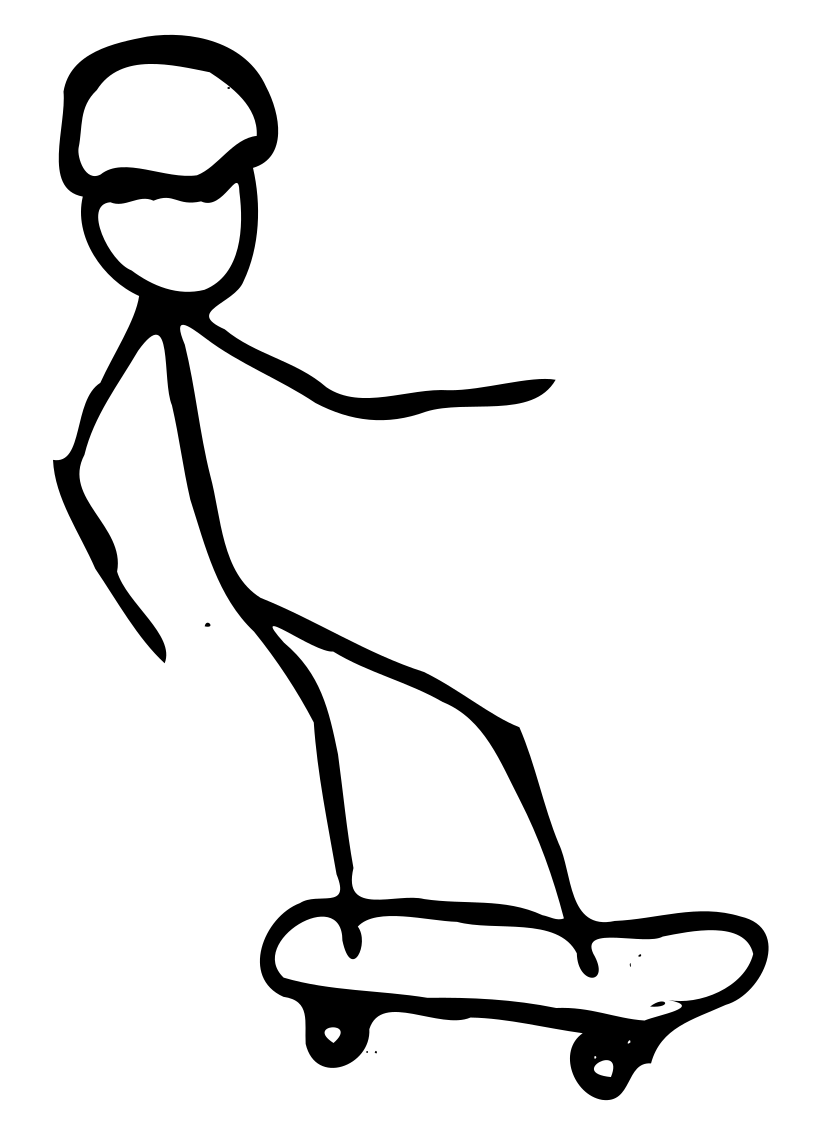
\includegraphics[width=0.5\textwidth]
            {../2012-ghentfpg-parallel/images/skate.pdf}}
    \end{picture}
\end{frame}

% The Haskell heap & `seq`
% ------------------------

\begin{frame}{Overview}
    \textbf{About Tsuru Capital} \\
    Why Haskell? \\
    Example: parsers \\
    Example: FRP \\
\end{frame}

\end{document}
